\documentclass[12pt,a4paper]{article}
\usepackage[utf8]{inputenc}
\usepackage[T1]{fontenc}
\usepackage{amsmath}
\usepackage{amsfonts}
\usepackage{amssymb}
\usepackage{multicol}
\usepackage{qrcode}
\usepackage{lmodern}
\usepackage{colortbl}%permet de griser les cases
\usepackage{tabularx, multirow}
%\usepackage{lscape}
\usepackage{xcolor}
%\usepackage{graphicx}
\usepackage{tikz,tkz-base}
\input{preambulemanu.sty}
\usepackage[left=2cm,right=2cm,top=2cm,bottom=2cm]{geometry}
\def\Oij{$\left(\text{O},~\vec{i},~\vec{j}\right)$}
\usepackage{fancyhdr}
\usepackage{MnSymbol,wasysym}

%Permet le code python sur lateX
\usepackage{minted}
\usemintedstyle{lovelace}



\begin{document}
\textbf{2nd} \hfill \textbf{Les fonctions affines} \hfill Lycée Jean Rostand\\
\trait 

\section{Généralité sur la fonction affine}



\begin{defi}



Une fonction $f$ est une fonction affine ssi $f$ est définie sur $\R$ par $f(x)=ax+b$\\ ($a$ et $b$ étant des nombres réels constants).\\
Le nombre $a$ est le coefficient directeur de la droite (pente) et $b$ est l'ordonnée à l'origine.\\
$\bullet$ si $a=0$ alors $f(x)=b$, alors $f$ est une fonction constante.\medskip\\
$\bullet$ si $b=0$ alors $f(x)=ax$, alors $f$ est une fonction linéaire.\medskip\\
Sa  représentation graphique est une droite.


\end{defi}

\subsection{Trouver graphiquement l'équation d'une fonction affine}

\begin{minipage}{0.85\textwidth}
Lien vidéo:
\url{https://youtu.be/yZSIxC-UtLg}
\end{minipage}
\begin{minipage}{0.2\textwidth}
\qrcode[height=2cm]{https://youtu.be/yZSIxC-UtLg}
\end{minipage}


Pour lire un coefficient directeur,on prend deux points sur la droite $A$ et $B$. Puis on se déplace de $A$ vers $B$ par la méthode de l'escalier. On en déduit le coefficient directeur:
$$\boxed{a=\dfrac{\text{déplacement vertical}}{\text{déplacement horizontal}}}$$

Pour l'ordonnée à l'origine, il suffit de lire l'ordonnée du point où la droite coupe l'axe des ordonnées



\begin{center}
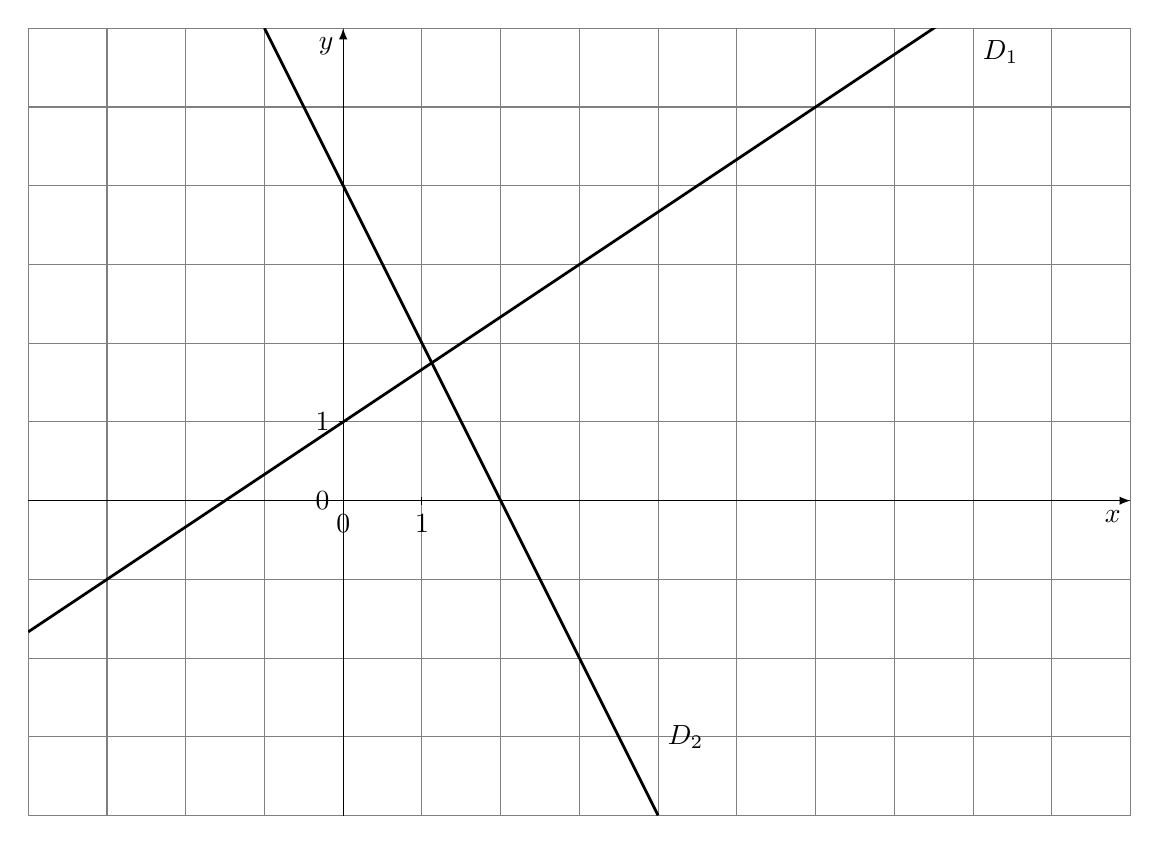
\begin{tikzpicture}[scale=1]

\draw [gray,xstep=1,ystep=1] (-4,-4) grid (10,6);
\draw [->,>=latex] (-4,0) -- (10,0) node [below left] {$x$};
\draw [->,>=latex] (0,-4) -- (0,6) node [below left] {$y$};

\foreach \x in {0,...,1}
\draw (\x,0.5mm) -- (\x,-0.5mm) node [below] {$\x$};
\foreach \y in {0,...,1}
\draw (0.5mm,\y) -- (-0.5mm,\y) node [left] {$\y$};

\clip (-4,-4) rectangle (10,6);
\draw [domain=-4:10,line width=1pt,samples=100] plot (\x,{2/3*\x+1});
\draw [domain=-1:4,line width=1pt,samples=100] plot (\x,{-2*\x+4});


\draw (8,5.7) node [right] {$\mathscr{D}_{1}$};
\draw (4,-3) node [right] {$\mathscr{D}_{2}$};

\end{tikzpicture}
\end{center}

\begin{mybox}{Exercice n°1}
Donner l'équation réduite des droites $\mathscr{D}_{1}$ et $\mathscr{D}_{2}$:

\end{mybox}

\begin{framed}
\vspace{2cm}
\end{framed}


\begin{mybox}{Exercice n°2}





Donner les équations réduites des différentes droites représentées ci-après:
\end{mybox}


\begin{center}
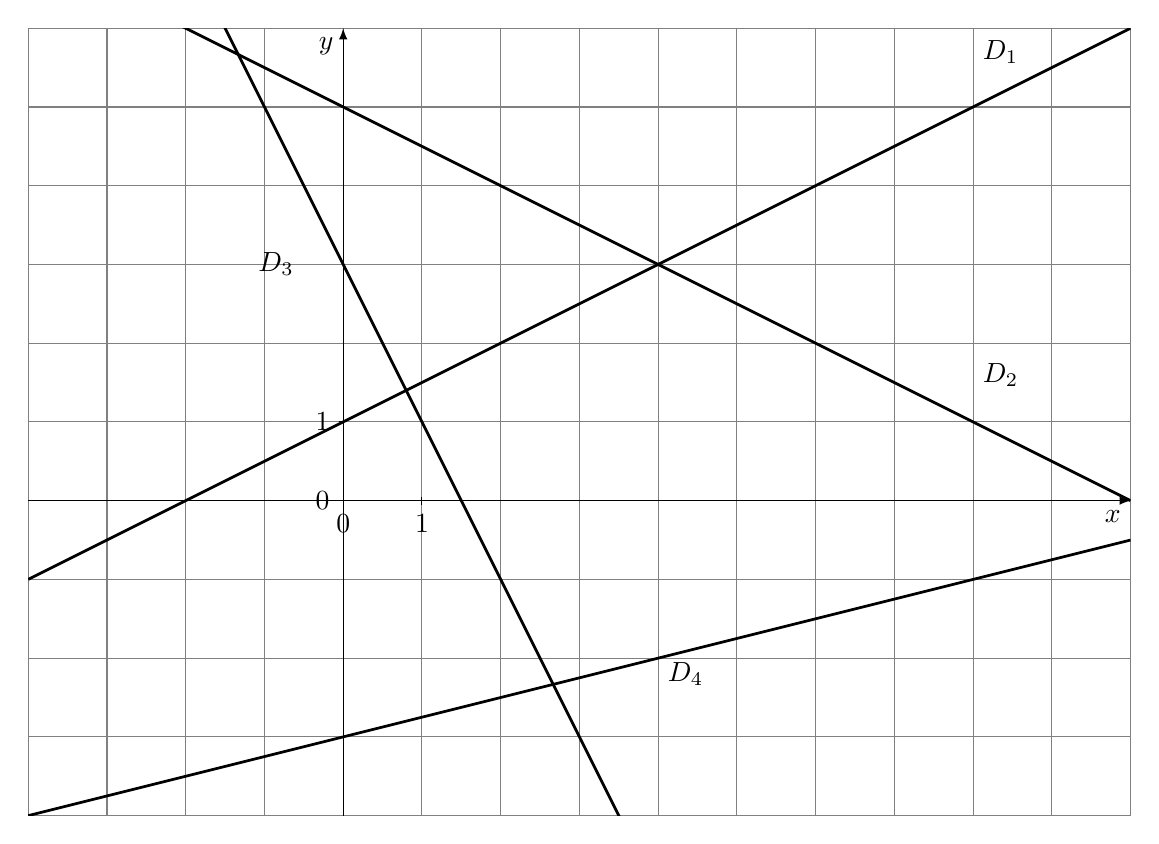
\begin{tikzpicture}[scale=1]

\draw [gray,xstep=1,ystep=1] (-4,-4) grid (10,6);
\draw [->,>=latex] (-4,0) -- (10,0) node [below left] {$x$};
\draw [->,>=latex] (0,-4) -- (0,6) node [below left] {$y$};

\foreach \x in {0,...,1}
\draw (\x,0.5mm) -- (\x,-0.5mm) node [below] {$\x$};
\foreach \y in {0,...,1}
\draw (0.5mm,\y) -- (-0.5mm,\y) node [left] {$\y$};

\clip (-4,-4) rectangle (10,6);
\draw [domain=-4:10,line width=1pt,samples=100] plot (\x,{(-2)*\x+3});
\draw [domain=-4:10,line width=1pt,samples=100] plot (\x,{1/2)*\x+1});
\draw [domain=-4:10,line width=1pt,samples=100] plot (\x,{(-1/2)*\x+5});
\draw [domain=-4:10,line width=1pt,samples=100] plot (\x,{(1/4)*\x-3});

\draw (8,5.7) node [right] {$\mathscr{D}_{1}$};
\draw (8,1.6) node [right] {$\mathscr{D}_{2}$};
\draw (-1.2,3) node [right] {$\mathscr{D}_{3}$};
\draw (4,-2.2) node [right] {$\mathscr{D}_{4}$};
\end{tikzpicture}
\end{center}

\begin{framed}
\vspace{5cm}
\end{framed}

\begin{mybox}{Exercice n°3}

Construire la représentation graphique de $f$, $g$, $h$ et $k$ définies par $f(x)=\frac{4}{5}x-3$, $g(x)=2x$, $h(x)=-\frac{4}{3}x+1$ et $k(x)=-3$

\end{mybox}
\begin{center}
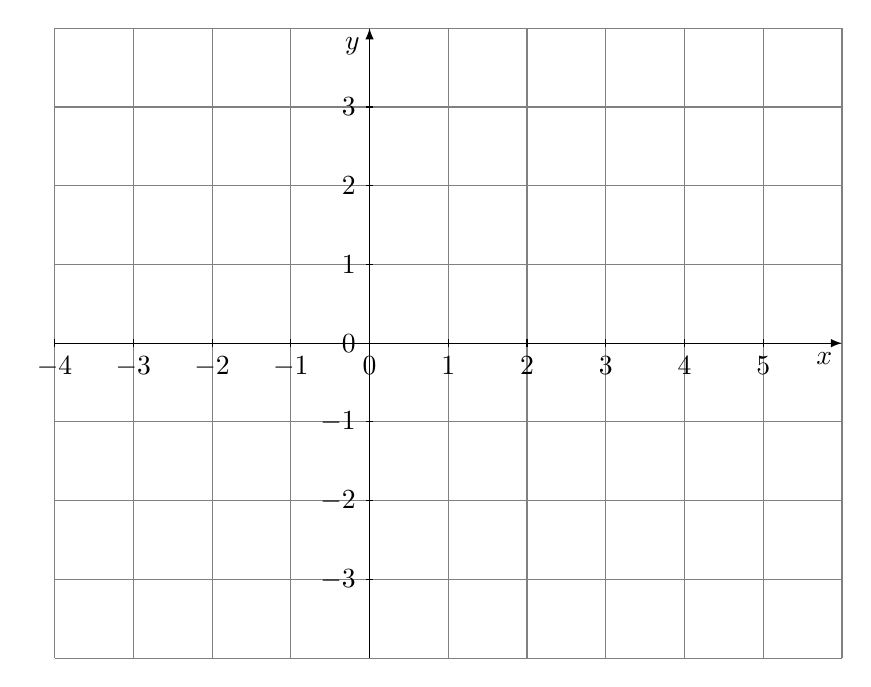
\begin{tikzpicture}[scale=1]
\draw [gray,xstep=1,ystep=1] (-4,-4) grid (6,4);
\draw [->,>=latex] (-4,0) -- (6,0) node [below left] {$x$};
\draw [->,>=latex] (0,-4) -- (0,4) node [below left] {$y$};

\foreach \x in {-4,...,5}
\draw (\x,0.5mm) -- (\x,-0.5mm) node [below] {$\x$};
\foreach \y in {-3,...,3}
\draw (0.5mm,\y) -- (-0.5mm,\y) node [left] {$\y$};

%\draw (0,0) node [below left] {$O$};

\clip (-4,-4) rectangle (6,4);
\end{tikzpicture}
\end{center}






\subsection{Trouver l'expression algébrique la fonction affine à partir de deux points}


\begin{minipage}{0.85\textwidth}
Lien vidéo:
\url{https://youtu.be/0jX7iPWCWI4}
\end{minipage}
\begin{minipage}{0.2\textwidth}
\qrcode[height=2cm]{https://youtu.be/0jX7iPWCWI4}
\end{minipage}

\begin{pro}
Si $A(x_A;y_A)$ et $B(x_B;y_B)$ sont deux points de la droite $\mathscr{D}$ représentant la fonction $f$ définie par $f(x)=ax+b$ alors:
$$\boxed{a=\dfrac{y_B-y_A}{x_B-x_A}}$$
\end{pro}


\begin{mybox}{Exercice n°3}


Déterminer une expression de la fonction affine telle que $f(3)=2$ et $f(2)=1$.
\begin{enumerate}
    \item Calculer le coefficient directeur de la droite $\mathscr{D}$.
    \item En déduire l'expression algébrique de la fonction affine.
\end{enumerate}

\end{mybox}

\begin{framed}
\vspace{2cm}
\end{framed}

\section{Tableau de signes et variations d'une fonction affine}

\subsection{Variation d'une fonction affine}
\begin{pro} Soit $f$ une fonction affine ($f(x)=ax+b$, $a$ étant le coefficient directeur)\medskip\\
$\bullet$ si $a>0$ alors $f$ est strictement croissante (la droite "monte").\medskip\\
$\bullet$ si $a<0$ alors $f$ est strictement décroissante (la droite "descend").\medskip
\end{pro}


\subsection{Tableau de signes d'une fonction affine}




\begin{minipage}{0.85\textwidth}
Lien vidéo:
\url{https://youtu.be/wYg6eNWd9V4}
\end{minipage}
\begin{minipage}{0.2\textwidth}
\qrcode[height=2cm]{https://youtu.be/wYg6eNWd9V4}
\end{minipage}









\begin{defi}
Soit $f$ une fonction affine de la forme $f(x)=ax+b$ alors $f(x)=0 \iff x=-\dfrac{b}{a}$.\\
\textbf{Règle des signes:}
\begin{center}
\begin{tikzpicture}
\tkzTabInit{$x$ / 1 , $f$ / 1}
           {$-\ii$,  $ -\dfrac{b}{a}$,   $+\ii$}
\tkzTabLine{ ,$signe de -a$,z,$signe de a$ , }
\end{tikzpicture}
\vspace{1cm}


\end{center}
\end{defi}



\begin{mybox}{Exercice n°4}

On considère la fonction affine $f$ telle que $f(x)=3x+2$.
Donner le tableau de signe de la fonction $f$.

\end{mybox}
\begin{framed}
\vspace{4cm}
\end{framed}

\subsection{Tableau de signes d'un produit de deux expressions affines }



\begin{minipage}{0.85\textwidth}
Lien vidéo 1:
\url{https://youtu.be/50CByVTP4ig}
\end{minipage}
\begin{minipage}{0.2\textwidth}
\qrcode[height=2cm]{https://youtu.be/50CByVTP4ig}
\end{minipage}


\vspace{0.5cm}


\begin{minipage}{0.85\textwidth}
Lien vidéo 2:
\url{https://youtu.be/qoNLr9NkvUE}
\end{minipage}
\begin{minipage}{0.2\textwidth}
\qrcode[height=2cm]{https://youtu.be/qoNLr9NkvUE}
\end{minipage}


\begin{mybox}{Exercice n°5}

On considère la fonction affine $f$ telle que $f(x)=(2x-5)(2x-1)$.
\begin{enumerate}
    \item Donner le tableau de signe de la fonction $f$.
    \item Résoudre l'inéquation $f(x)\geq 0$
\end{enumerate}


\end{mybox}
\begin{framed}
\vspace{4cm}
\end{framed}














\subsection{Tableau de signes d'un quotient de deux expressions affines }


\begin{minipage}{0.85\textwidth}
Lien vidéo:
\url{https://youtu.be/Vitm29q8AEs}
\end{minipage}
\begin{minipage}{0.2\textwidth}
\qrcode[height=2cm]{https://youtu.be/Vitm29q8AEs}
\end{minipage}


\begin{mybox}{Exercice n°5}

On considère la fonction affine $f$ telle que $f(x)=\frac{-2x+8}{3x+5}$.
\begin{enumerate}
    \item Donner le tableau de signe de la fonction $f$.
    \item Résoudre l'inéquation $f(x)\geq 0$
\end{enumerate}


\end{mybox}
\begin{framed}
\vspace{4cm}
\end{framed}










\end{document}
